\documentclass[11pt,a4paper]{article}
\usepackage[titletoc,toc,title]{appendix}
\usepackage{tikz}
\usetikzlibrary{matrix,chains,positioning,decorations.pathreplacing,arrows}
\usepackage[nottoc,notlot,notlof]{tocbibind}
% Modèle de rapport de stage et conseils de rédaction, mise en page...
% L. Bellon, avril 2010
\usepackage{listings}
% définition des marges du document
\setlength{\topmargin}{0cm}
\setlength{\headheight}{0.4cm}
\setlength{\headsep}{0.8cm}
\setlength{\footskip}{1cm}
\setlength{\textwidth}{17cm}
\setlength{\textheight}{25cm}
\setlength{\voffset}{-1.5cm}
\setlength{\hoffset}{-0.5cm}
\setlength{\oddsidemargin}{0cm}
\setlength{\evensidemargin}{0cm}
\usepackage{subfig}
% quelques package utiles
\usepackage{graphicx} % inclusion des figures
\usepackage{tikz}
\usepackage{amsmath} % collection de symboles mathématiques
\usepackage{amssymb} % collection de symboles mathématiques


\usepackage{pdfpages}
\makeatletter
\def\BState{\State\hskip-\ALG@thistlm}
\makeatother

%\usepackage[applemac]{inputenc}       % utilisation directe des caractères accentués sur mac
\usepackage[utf8]{inputenc}       % utilisation directe des caractères accentués sur pc
\usepackage[T1]{fontenc} % codage moderne des caractères sous Latex

\usepackage[francais]{babel}           % style français

\usepackage{tabularx} % gestion avancée des tableaux

\usepackage{psfrag} % remplacement du texte d'une figure ps par du texte latex
\usepackage{sistyle} % mise en forme des unités

\usepackage{eurosym} % symbole €
\def\€{\euro{}}

\usepackage{color} % gestion de différentes couleurs

\definecolor{linkcolor}{rgb}{0,0,0.6} % définition de la couleur des liens pdf
\usepackage[ pdftex,colorlinks=true,
pdfstartview=FitV,
linkcolor= linkcolor,
citecolor= linkcolor,
urlcolor= linkcolor,
hyperindex=true,
hyperfigures=false]
{hyperref} % fichiers pdf 'intelligents', avec des liens entre les références, etc.

\usepackage{fancyhdr} % entêtes et pieds de pages personnalisés

% définition de l'entête et du pied de page
\pagestyle{fancy}
\fancyhead[L]{\scriptsize \textsc{Dicotomix}}
\fancyhead[R]{\scriptsize \textsc{Équipe Dicotomix}}
\fancyfoot[C]{ \thepage}

% commande d'annulation du correcteur typographique du package [francais]{babel} qui force l'espace avant ':' (parfois utile pour la bibliographie)
\makeatletter
\@ifpackageloaded{babel}%
        {\newcommand{\nospace}[1]{{\NoAutoSpaceBeforeFDP{}#1}}}%  % !! double {{}} pour cantonner l'effet à l'argument #1 !!
        {\newcommand{\nospace}[1]{#1}}
\makeatother

% commande de déplacement d'un objet
\newcommand{\drawat}[3]{\makebox[0pt][l]{\raisebox{#2}{\hspace*{#1}#3}}}

\usepackage{amsthm}
\theoremstyle{plain}
\newtheorem{thm}{Théorème}[section] % reset theorem numbering for each chapter

\theoremstyle{definition}
\newtheorem{defn}[thm]{Définition} % definition numbers are dependent on theorem numbers

\begin{document}

% Pour faciliter la mise en forme de la page du titre, on supprime l'indentation automatique en début de paragraphe
\setlength{\parindent}{0pt}

% Pas d'en-tête ni de pied pour la première page
\thispagestyle{empty}


\includegraphics[height=2cm]{logoens.eps} \hfill \includegraphics[height=2cm]{logoucbl.eps} \hfill \includegraphics[height=2cm]{logounivlyon.eps}

\vspace{0.5cm}

\begin{tabularx}{\textwidth}{@{} l X l @{} }
{\sc Master d'informatique fondamentale} & & U.E Projet intégré\\
{\it École Normale Supérieure de Lyon} & & Équipe Dicotomix\ \\
{\it Université Claude Bernard Lyon I} 
\end{tabularx}

\begin{center}


\vspace{1.5cm}

\rule[11pt]{5cm}{0.5pt}

\textbf{\huge Dicotomix}

\rule{5cm}{0.5pt}
\vspace{0.5cm}


\includegraphics[scale=0.7]{icon.eps}

\vspace{0.5cm}

M.Guy, E.Hazard, E.Kerinec,\\ F.Lécuyer, P.Mangold, A.Martin,\\ R.Pellerin, N.Pinson, A.Słowik, T.Stérin

\vspace{1.5cm}

\parbox{15cm}{\small
\textbf{Résumé} : \it Les réseaux de neurones récurrents sont des modèles aptes à apprendre et à générer des séquences temporelles. Ces réseaux se déclinent en plusieurs variantes dont les deux principales sont Vanilla et LSTM. À travers un exemple concret d'inférence grammaticale on constate la faiblesse des Vanilla à exploiter des dépendances temporelles longues. Sur la base de ces résultats expérimentaux on remet en cause l'importance de la raison la plus souvent invoquée dans la littérature pour expliquer cette faiblesse. On propose une autre explication que l'on conjuge avec l'introduction d'une mesure de la capacité de mémoire d'un modèle récurrent. On confronte cette mesure à la théorie des Echo States Networks qui aborde ces questions de mémoire différemment. Forts de ces expériences on applique les techniques décrites à la génération de musique à travers les chorals de Bach.

} %fin de la commande \parbox du résumé


\vspace{0.5cm}

\parbox{15cm}{
\textbf{Mots clefs} : \it RNNs, Mémoire, Echo States Networks, Musique
} %fin de la commande \parbox des mots clefs

\vspace{1.5cm}

\parbox{15cm}{


\includegraphics{logo-hcl-plein_2995-bleu.jpg} \hfill

\includegraphics[scale=0.15]{ARS-Auvergne-Rhone-Alpes.jpg}
} %fin de la commande \parbox encadrant / laboratoire d'accueil

\vspace{0.5cm}
\vspace{0.5cm}
\end{center}

\vfill
\hfill \today
\newpage
% Pas d'entête ni de pied pour la page de sommaire
\thispagestyle{empty}
\section*{Remerciements}

\tableofcontents

\newpage
\section{Introduction}

Le Locked-In Syndrome (\textbf{LIS}) est un état neurologique qui prive les patients de la quasi-totalité de leurs capacités motrices, ils ne peuvent ni bouger ni parler,
sans altérer \textit{a priori} leurs capacités cognitives. Aussi appelé syndrome d'enfermement, les patients se retrouvent prisonniers de leur corps.
Cette maladie a été notamment été présentée au grand public à travers \textit{Le scaphandre et le papillon} retraçant le combat de Jean-Dominique Bauby pour communiquer.

\paragraph{} Communiquer, c'est cette problématique qui à l'origine du projet Dicotomix. Comment améliorer les moyens de communications des patients atteints de LIS ? Plus généralement, la rencontre avec le monde hospitalier nous a fait comprendre que ce problème est plus général car il concerne d'autres maladies, comme la maladie
de Charcot ou sclérose latérale amyotrophique (\textbf{SLA}). 

\paragraph{} Ce rapport a donc pour objectif de présenter les différentes solutions pensées par notre équipe pour répondre à ce problème. C'est grâce au monde hospitalier que 
nous avons pu confronter nos "idées de laboratoire" aux besoins réels des patients et du monde médical. Cette confrontation a constamment guidé notre démarche et a conduit à notre
réalisation principale, le logiciel Dicotomix.

\paragraph{} Enfin, nous avons eu la chance de pouvoir faire tester notre logiciel à un patient LIS et une patiente SLA au cours d'une étude pilote menées avec les Hospices Civiles de Lyon.
Cet aboutissement, très intense humainement, redessinant, encore une fois, les contours du projet.
De sa genèse à l'étude pilote, c'est l'aventure humaine et scientifique du projet Dicotomix.


\section{Genèse du projet}
\section{La solution Dicotomix}
\section{L'étude pilote}
\section{Conclusion}

\appendix
\section{Intervenants extérieurs et chronologie détaillée}
\section{Étude comparative de la solution Dicotomix}
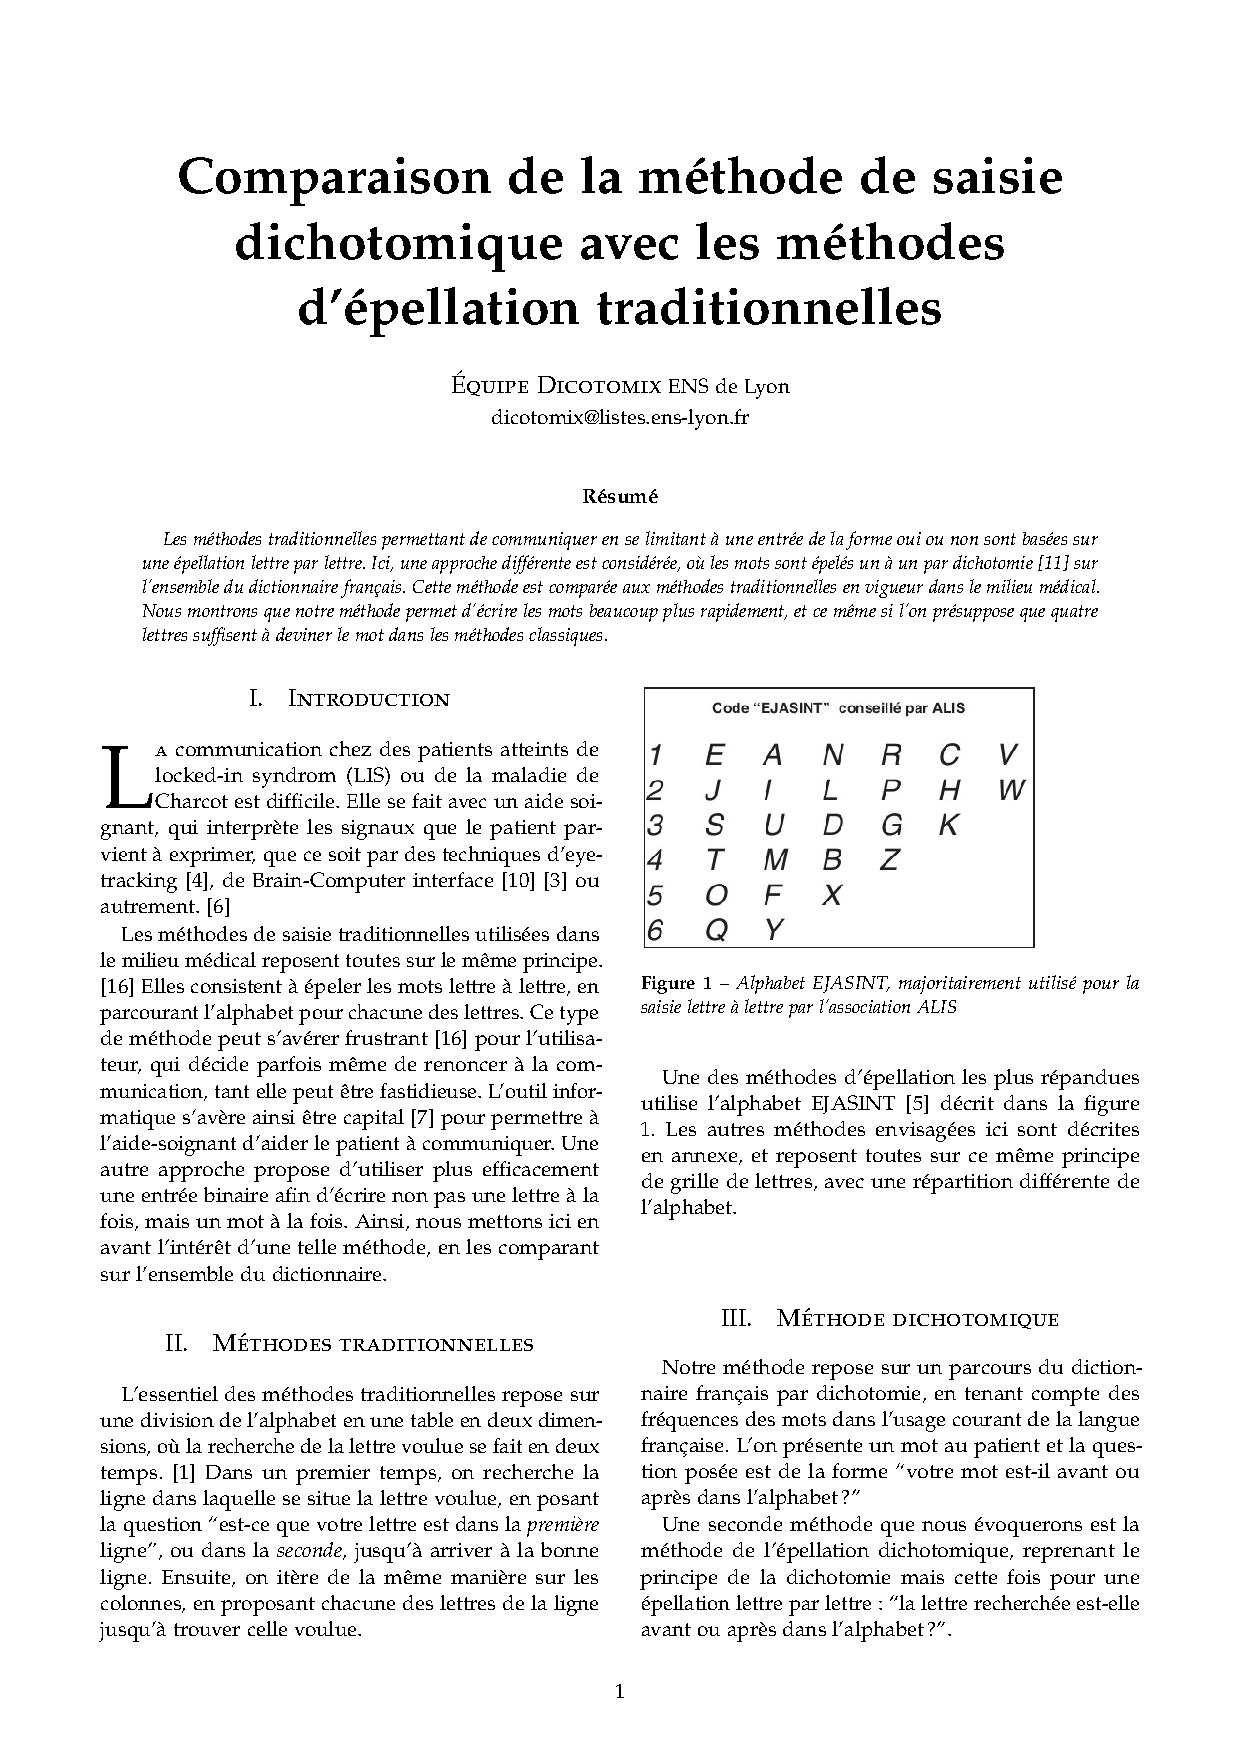
\includepdf[pages=-]{comparison.pdf}
\section{Tutoriel d'utilisation de Dicotomix}
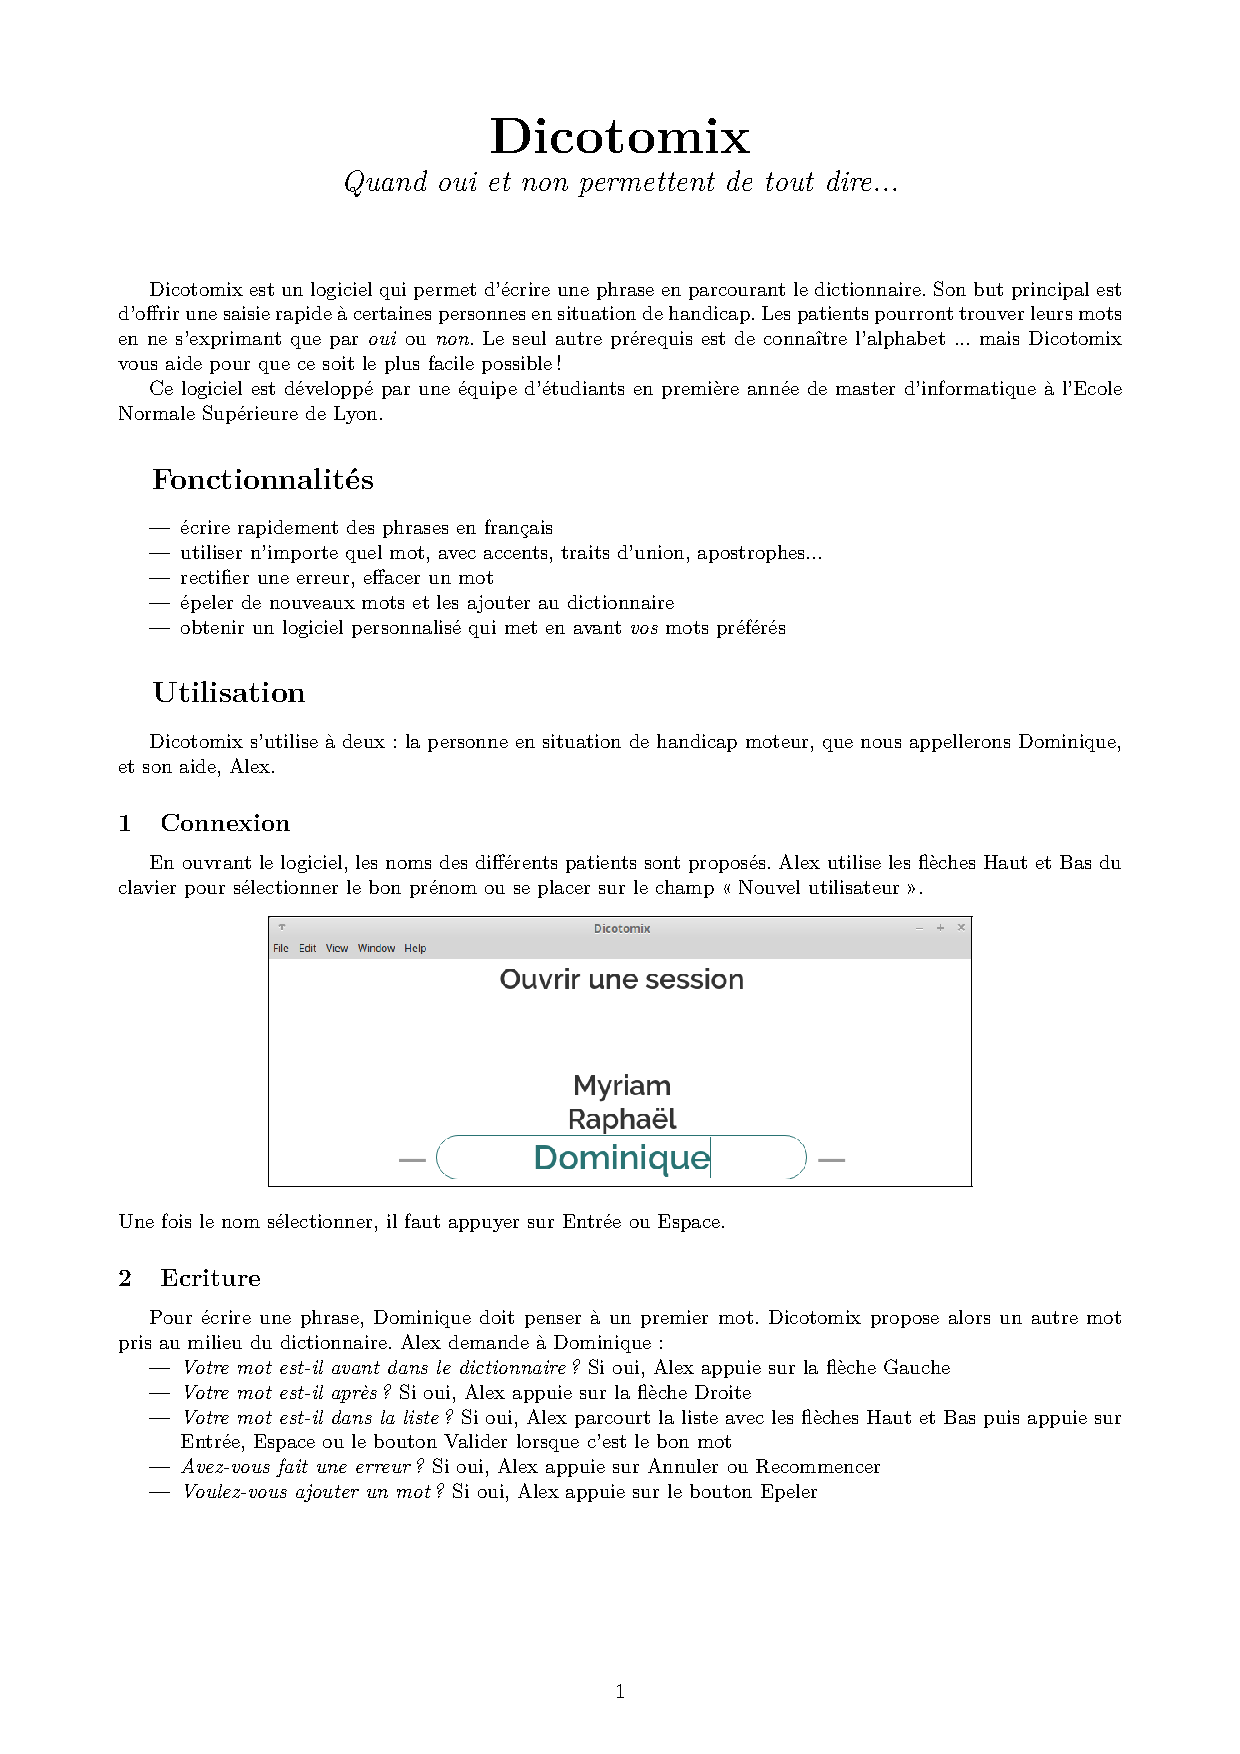
\includepdf[pages=-]{tutoriel.pdf}
\end{document}